
%(BEGIN_QUESTION)
% Copyright 2010, Tony R. Kuphaldt, released under the Creative Commons Attribution License (v 1.0)
% This means you may do almost anything with this work of mine, so long as you give me proper credit

Suppose this three-phase AC electric motor refuses to start as it should when the transistor turns on.  A voltmeter subsequently connected between test points {\bf E} and {\bf F} in this circuit registers 480 volts with the transistor biased to be in the ``on'' state:

$$\includegraphics[width=15.5cm]{i04674x01.eps}$$

Identify the likelihood of each specified fault for this circuit.  Consider each fault one at a time (i.e. no coincidental faults), determining whether or not each fault could independently account for {\it all} measurements and symptoms in this circuit.

% No blank lines allowed between lines of an \halign structure!
% I use comments (%) instead, so that TeX doesn't choke.

$$\vbox{\offinterlineskip
\halign{\strut
\vrule \quad\hfil # \ \hfil & 
\vrule \quad\hfil # \ \hfil & 
\vrule \quad\hfil # \ \hfil \vrule \cr
\noalign{\hrule}
%
% First row
{\bf Fault} & {\bf Possible} & {\bf Impossible} \cr
%
\noalign{\hrule}
%
% Another row
Transistor failed open &  &  \cr
%
\noalign{\hrule}
%
% Another row
Motor winding(s) failed open &  &  \cr
%
\noalign{\hrule}
%
% Another row
All 15 A fuses blown &  &  \cr
%
\noalign{\hrule}
%
% Another row
Transistor failed shorted &  &  \cr
%
\noalign{\hrule}
%
% Another row
Relay coil failed open &  &  \cr
%
\noalign{\hrule}
%
% Another row
0.5 amp fuse blown &  &  \cr
%
\noalign{\hrule}
%
% Another row
24 VDC source dead &  &  \cr
%
\noalign{\hrule}
} % End of \halign 
}$$ % End of \vbox

\vfil 

\underbar{file i04674}
\eject
%(END_QUESTION)





%(BEGIN_ANSWER)

% No blank lines allowed between lines of an \halign structure!
% I use comments (%) instead, so that TeX doesn't choke.

$$\vbox{\offinterlineskip
\halign{\strut
\vrule \quad\hfil # \ \hfil & 
\vrule \quad\hfil # \ \hfil & 
\vrule \quad\hfil # \ \hfil \vrule \cr
\noalign{\hrule}
%
% First row
{\bf Fault} & {\bf Possible} & {\bf Impossible} \cr
%
\noalign{\hrule}
%
% Another row
Transistor failed open & $\surd$ &  \cr
%
\noalign{\hrule}
%
% Another row
Motor winding(s) failed open & $\surd$ &  \cr
%
\noalign{\hrule}
%
% Another row
All 15 A fuses blown &  & $\surd$ \cr
%
\noalign{\hrule}
%
% Another row
Transistor failed shorted &  & $\surd$ \cr
%
\noalign{\hrule}
%
% Another row
Relay coil failed open & $\surd$ &  \cr
%
\noalign{\hrule}
%
% Another row
0.5 amp fuse blown & $\surd$ &  \cr
%
\noalign{\hrule}
%
% Another row
24 VDC source dead & $\surd$ &  \cr
%
\noalign{\hrule}
} % End of \halign 
}$$ % End of \vbox

%(END_ANSWER)





%(BEGIN_NOTES)

{\bf This question is intended for exams only and not worksheets!}.

%(END_NOTES)

